\section{Database}
\subsection{Descrizione}
Per garantire la semplicità di gestione e la velocità di esecuzione delle query nel database sono presenti solo 3 tabelle: Users, Products e Transactions. Queste sono il minimo indispensabile per la creazione di un e-commerce funzionante. Il database sarà collocato nel data server che conterrà anche le immagini di profilo degli utenti e quelle legate ai prodotti. Quella riportata nel modello E/R è la prima versione del database che permette di caricare un'unica immagine per prodotto, nelle versioni successive verranno introdotti aggiornamenti graduali paralleli allo sviluppo completo del sito web. 
\medskip

La tabella Users contiene le informazioni base necessarie per l'utilizzo della piattaforma: ID utente, nome utente, password, email identificativa, città di residenza, immagine di profilo, salt per la generazione dell'hash della password, api key per eseguire richieste tramite l'API e quantità di green coin posseduti. 
\medskip

La tabella Products contiene invece i seguenti campi: ID prodotto, nome prodotto, descrizione prodotto, immagine del prodotto, disponibilità (per tenere traccia dei prodotti anche dopo la loro vendita o la rimozione dal mercato), data dell'ultimo aggiornamento apportato al prodotto e ID utente proprietario del prodotto. 
\medskip

La tabella Transactions contiene le transazioni effettuate tra gli utenti e ha i seguenti campi: ID transazione, ID prodotto scambiato, ID utente proprietario del prodotto al momento dello scambio (campo necessario per tenere traccia dei cambi di proprietà e delle transazioni anche dopo che queste si sono concluse), ID utente acquirente, stato della transazione (può essere "In Corso", "Completata Con Successo" o "Completata Senza Successo") e data dell'ultimo aggiornamento relativo alla transazione. 
\subsection{Modello E/R}
\begin{figure}[ht]
    \centering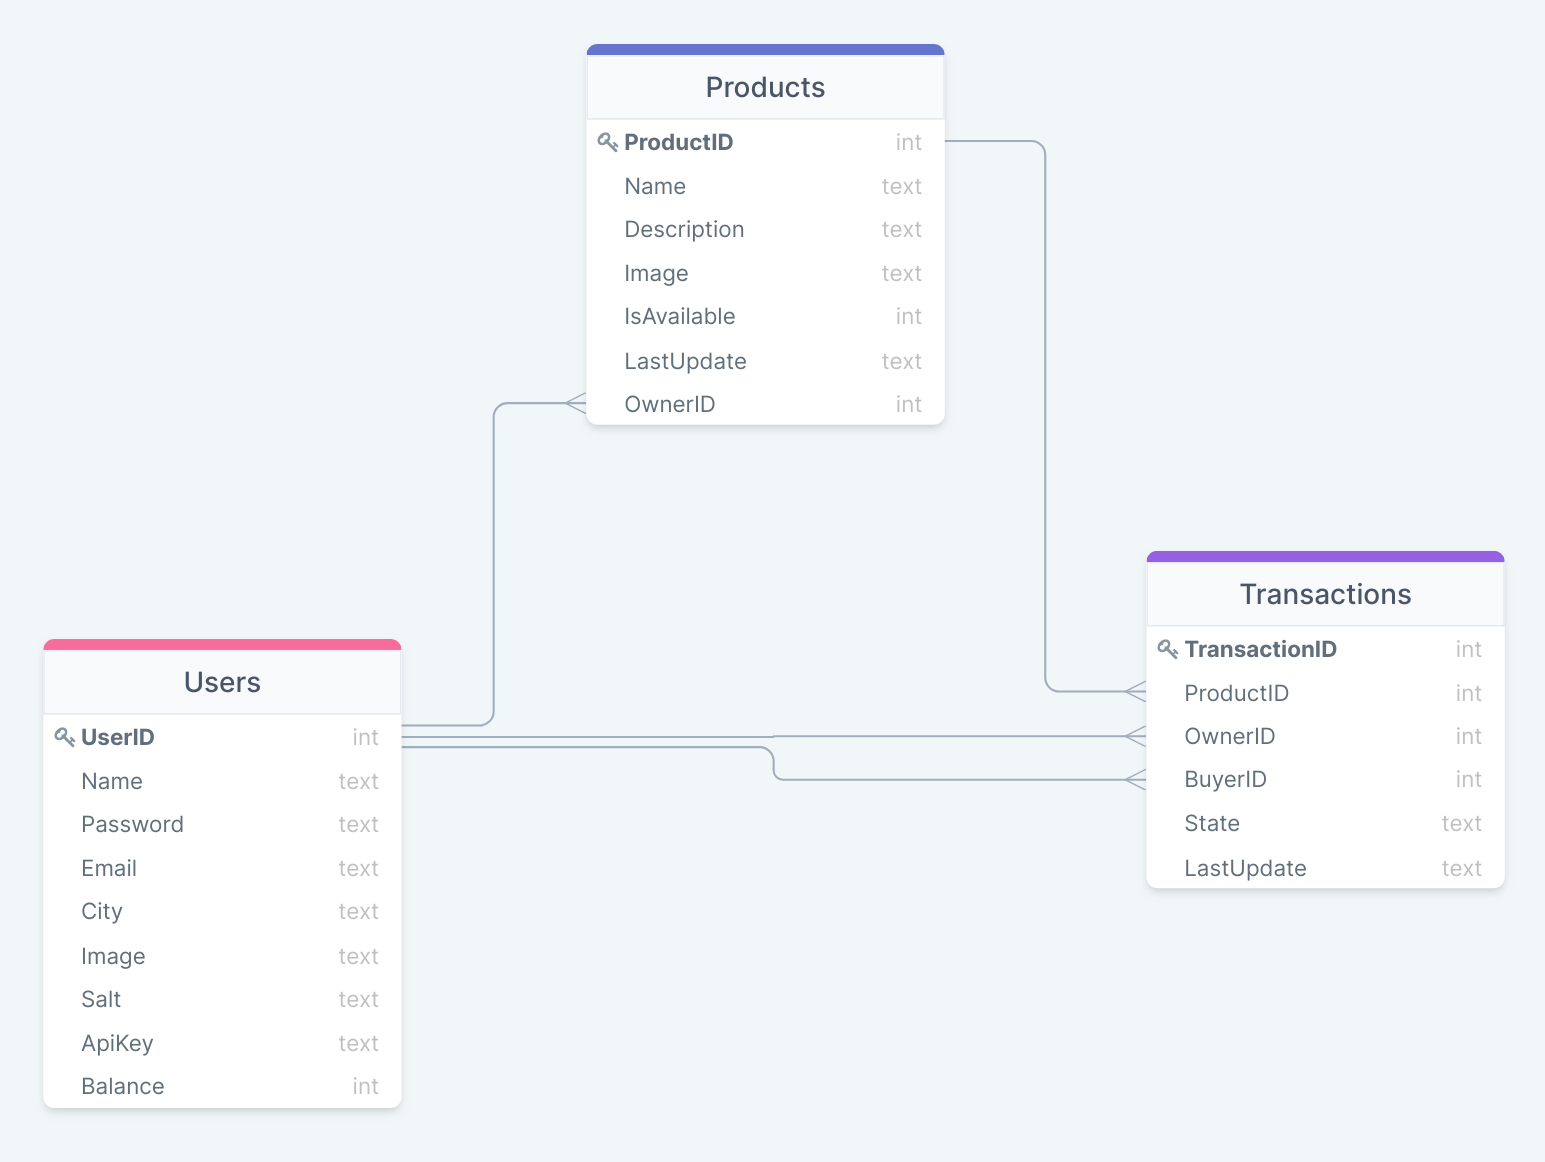
\includegraphics[scale=0.29]{images/modello_e_r.png}
    \caption{Modello E/R del database}
\end{figure}
\subsection{Modello logico}
\begin{figure}[ht]
    \centering\begin{tabular}{ |l|c|l| } 
    \hline
    \multicolumn{3}{|c|}{\large\textbf{Users}} \\
    \hline
    \textbf{Nome Campo} & \textbf{Tipo} & \textbf{Note} \\
    \hline
    UserID & INTEGER & NOT NULL, PK, AUTOINCREMENT \\
    Name & TEXT & NOT NULL \\
    Password & TEXT & NOT NULL \\
    Email & TEXT & NOT NULL \\
    City & TEXT & NOT NULL \\
    Image & TEXT & NOT NULL \\
    Salt & TEXT & NOT NULL \\
    ApiKey & TEXT & NOT NULL \\
    Balance & INTEGER & NOT NULL \\
    \hline
    \end{tabular}
    \caption{Tabella Users parte del modello logico del database}
\end{figure}
\begin{figure}[ht]
    \centering\begin{tabular}{ |l|c|l| } 
    \hline
    \multicolumn{3}{|c|}{\large\textbf{Products}} \\
    \hline
    \textbf{Nome Campo} & \textbf{Tipo} & \textbf{Note} \\
    \hline
    ProductID & INTEGER & NOT NULL, PK, AUTOINCREMENT \\
    Name & TEXT & NOT NULL \\
    Description & TEXT & NOT NULL \\
    Image & TEXT & NOT NULL \\
    IsAvailable & INTEGER & NOT NULL \\
    LastUpdate & TEXT & NOT NULL \\
    OwnerID & INTEGER & NOT NULL, FK(Users) \\
    \hline
    \end{tabular}
    \caption{Tabella Products parte del modello logico del database}
\end{figure}
\begin{figure}[ht]
    \centering\begin{tabular}{ |l|c|l| } 
    \hline
    \multicolumn{3}{|c|}{\large\textbf{Transactions}} \\
    \hline
    \textbf{Nome Campo} & \textbf{Tipo} & \textbf{Note} \\
    \hline
    TransactionID & INTEGER & NOT NULL, PK, AUTOINCREMENT \\
    ProductID & INTEGER & NOT NULL, FK(Products) \\
    OwnerID & INTEGER & NOT NULL, FK(Users) \\
    BuyerID & INTEGER & NOT NULL, FK(Users) \\
    State & TEXT & NOT NULL \\
    LastUpdate & TEXT & NOT NULL \\
    \hline
    \end{tabular}
    \caption{Tabella Transactions parte del modello logico del database}
\end{figure}
\clearpage
\subsection{Entity Framework Core}
Il database è stato generato automaticamente da Entity Framework Core a partire dai modelli scritti in C\# e inseriti nel progetto (generazione code-first). I modelli inseriti devono essere riportati nel DbContext indicato nel file Startup.cs, il database context si occupa quindi di descrive il database e le tabelle che lo compongono, quest'ultime vengono invece descritte dai modelli indicati nel database context. La nomenclatura dei modelli comprende l'espressione DTO (Data Transfer Object) in quanto queste classi vengono usate per il trasferimento di dati dagli utenti al database. 
\bigskip

\textbf{MainDbContext.cs}
\lstinputlisting{content/code/MainDbContext.cs}
\bigskip

\textbf{UserDTO.cs}
\lstinputlisting{content/code/UserDTO.cs}
\bigskip

\textbf{ProductDTO.cs}
\lstinputlisting{content/code/ProductDTO.cs}
\bigskip

\textbf{TransactionDTO.cs}
\lstinputlisting{content/code/TransactionDTO.cs}

\subsection{Query}
Usando Entity Framework Core per la creazione e la gestione del database le query possono essere scritte con la sintassi sviluppata da Microsoft chiamata LINQ, alternativamente possono essere anche usati i metodi appositi inclusi nella libreria Microsoft dedicata (Microsoft.EntityFrameworkCore). Nel progetto ho scelto di usare la libreria Microsoft dedicata in quanto è la più veloce e quella che richiede meno l'intervento del programmatore, evitando quindi errori semplici di distrazione. 
\bigskip

\textbf{Query LINQ}
\lstinputlisting{content/code/linq.cs}
\bigskip

\textbf{Query con metodi}
\lstinputlisting{content/code/libreria.cs}